\documentclass[../main/main.tex]{subfiles}

\begin{document}

\chapter{利用例と参照方法}
\label{chap:examples}

この章では、博士論文でよく使用される各種参照方法と図表の挿入方法について、具体的な例を示します。

\section{cleverefパッケージによる参照}
\label{sec:basic_refs}

\subsection{基本的な参照}
\label{subsec:basic_refs}

cleverefパッケージを使用することで、参照が自動的に適切な形式で表示されます。

\begin{itemize}
    \item 章の参照:\cref{chap:examples}で示したように
    \item 節の参照:\cref{sec:basic_refs}で説明した通り
    \item 図の参照:\cref{fig:sample_plot}に示されている
    \item 表の参照:\cref{tab:sample_table}を参照してください
    \item 式の参照:\cref{eq:sample_equation}から分かるように
\end{itemize}

\subsection{複数の参照}

複数の項目を同時に参照することも可能です:

\begin{itemize}
    \item 図と表の組み合わせ:\cref{fig:sample_plot,tab:sample_table}
    \item 複数の式:\cref{eq:sample_equation,eq:eq1}
    \item 章と節の組み合わせ:\cref{sec:basic_refs,subsec:basic_refs}
\end{itemize}

\section{図表の挿入方法}

\subsection{図の挿入}

図\ref{fig:sample_plot}は、サンプルプロットを示しています。

\begin{figure}[htbp]
    \centering
    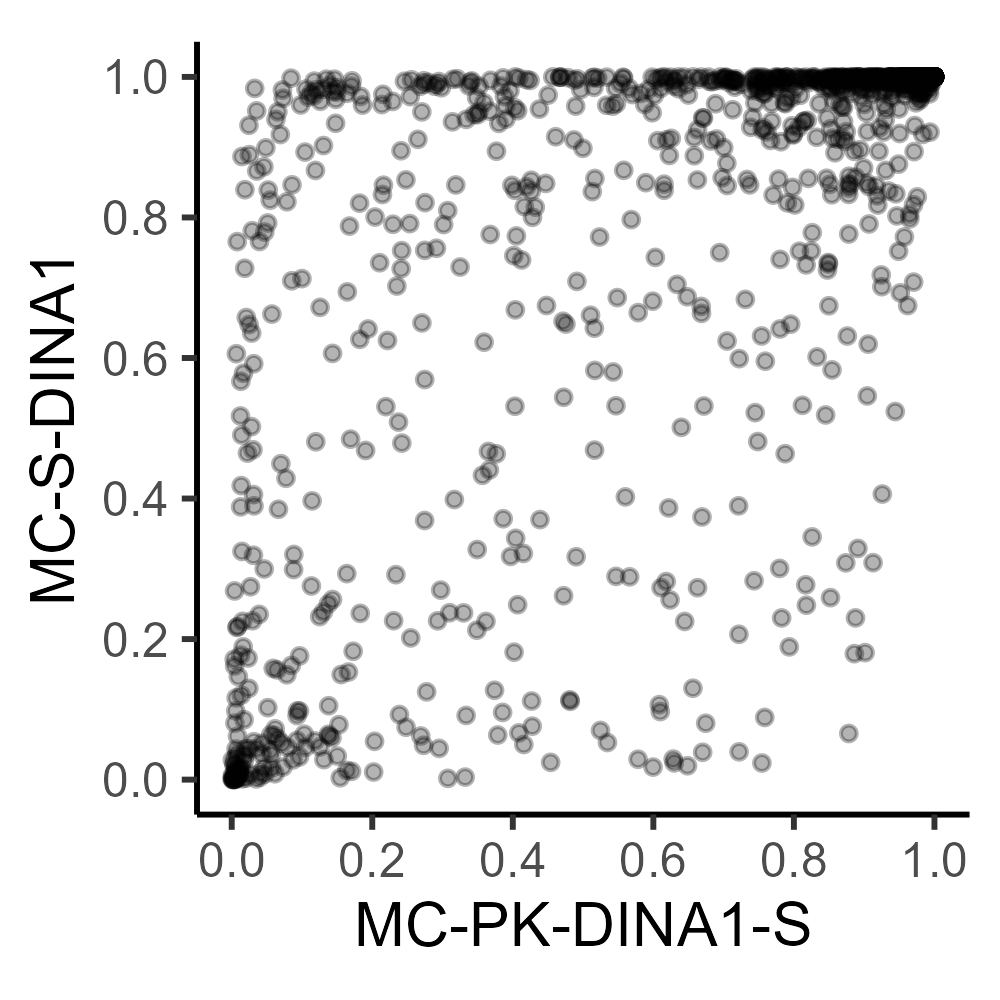
\includegraphics[width=0.8\textwidth]{../images/Chap_A/demo_plot.png}
    \caption{サンプルプロットの例}
    \label{fig:sample_plot}
\end{figure}

\subsection{表の挿入}

表\ref{tab:sample_table}は、サンプルデータを示しています。

\begin{table}[htbp]
    \centering
    \caption{サンプルデータ表}
    \label{tab:sample_table}
    \begin{tabular}{lcc}
        \hline
        項目 & 値1 & 値2 \\
        \hline
        A & 1.23 & 4.56 \\
        B & 2.34 & 5.67 \\
        C & 3.45 & 6.78 \\
        \hline
    \end{tabular}
\end{table}

\subsection{サブキャプション付き図}

複数の図を組み合わせる場合:

\begin{figure}[htbp]
    \centering
    \begin{subfigure}[b]{0.45\textwidth}
        \centering
        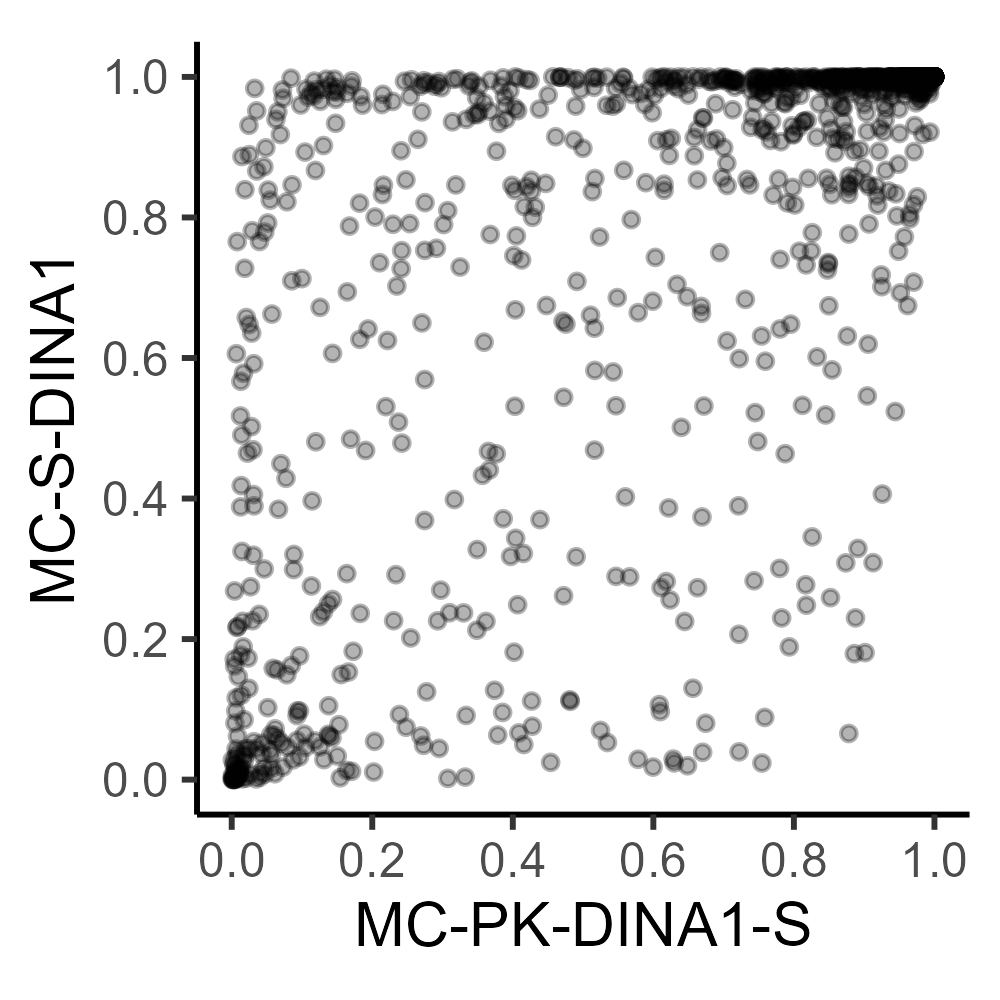
\includegraphics[width=\textwidth]{../images/Chap_A/demo_plot.png}
        \caption{図A}
        \label{fig:subplot_a}
    \end{subfigure}
    \hfill
    \begin{subfigure}[b]{0.45\textwidth}
        \centering
        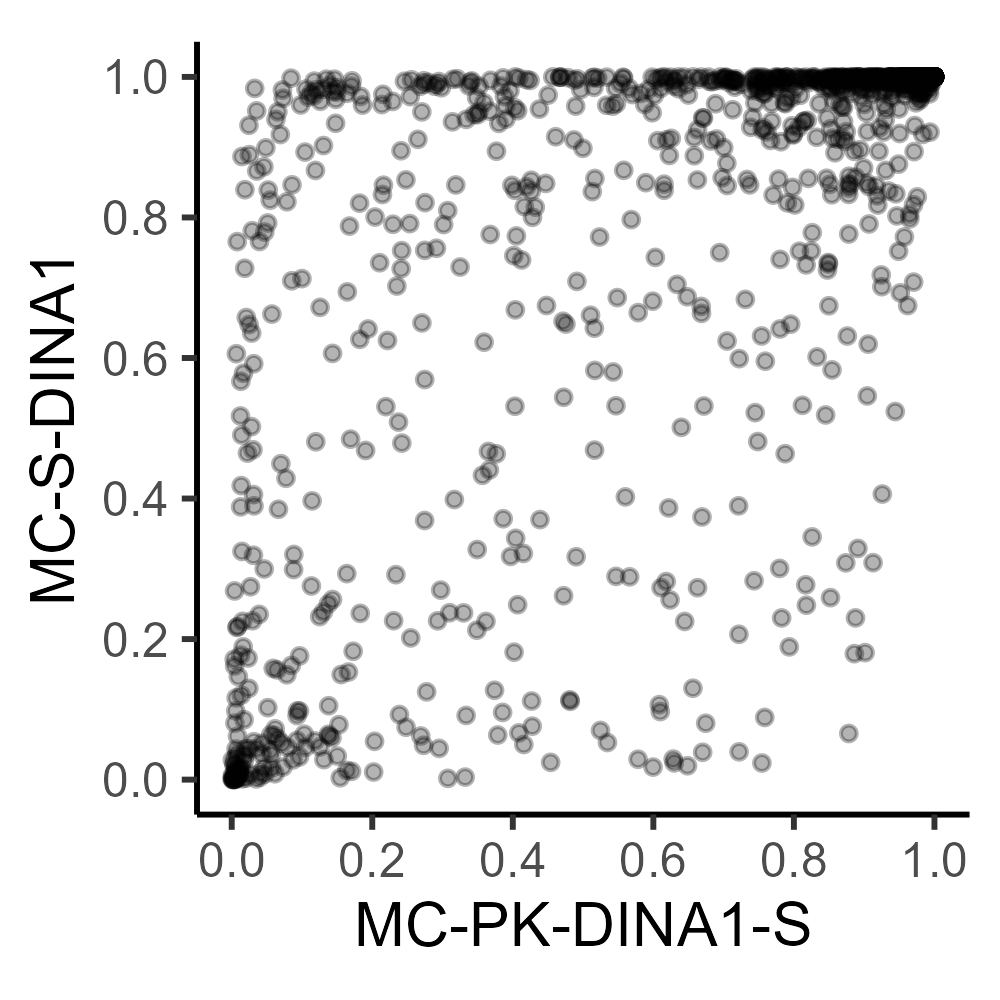
\includegraphics[width=\textwidth]{../images/Chap_A/demo_plot.png}
        \caption{図B}
        \label{fig:subplot_b}
    \end{subfigure}
    \caption{サブキャプション付き図の例}
    \label{fig:subplots}
\end{figure}

\section{数式の参照}

\subsection{基本的な数式}

以下の数式を考えます:

\begin{equation}
    E = mc^2
    \label{eq:sample_equation}
\end{equation}

\cref{eq:sample_equation}は、アインシュタインの質量エネルギー等価式です。

\subsection{複数の数式}

連立方程式の例:

\begin{align}
    x + y &= 10 \label{eq:eq1} \\
    x - y &= 2 \label{eq:eq2}
\end{align}

\cref{eq:eq1,eq:eq2}から、$x = 6$、$y = 4$が得られます。

\section{引用の仕方}

\subsection{基本的な引用}

\textcite{arai2020japanese}は、思考力を測る多枝選択式問題について研究を行いました。

\textcite{Black1998-yt}によると、形成的評価は学習に重要な役割を果たします。

\parencite{arai2020japanese}は、思考力を測る多枝選択式問題について研究を行いました。
\textcite{arai2020japanese}は、思考力を測る多枝選択式問題について研究を行いました。

\subsection{複数の引用}

複数の研究を同時に引用する場合:

\textcite{arai2020japanese}と\textcite{Black1998-yt}は、評価に関する重要な研究を行いました。

\subsection{括弧内引用}

\parencite{arai2020japanese}の研究では、思考力測定の重要性が指摘されています。

\parencite{Black1998-yt,arai2020japanese}の研究結果は、形成的評価の有効性を示しています。

\subsection{ページ指定付き引用}

\parencite[p.~15]{arai2020japanese}で述べられているように、思考力測定には注意深い設計が必要です。

\subsection{著者名を含む引用}

\textcite{arai2020japanese}は、\parencite[p.~20]{arai2020japanese}で詳細に説明しています。

\subsection{テキスト内引用}

\cite{arai2020japanese}の研究は、思考力測定の新しいアプローチを提案しています。

\cite{Black1998-yt,arai2020japanese}の研究結果は、形成的評価の有効性を示しています。

\subsection{脚注付き引用}

\footcite{arai2020japanese}の研究では、思考力測定の重要性が指摘されています。

\subsection{括弧内著者名引用}

\parencite{arai2020japanese}は、思考力測定の新しいアプローチを提案しています。

\section{章をまたいだ参照}

\subsection{他の章への参照}

\cref{chap:examples}で示した例は、\cref{sec:basic_refs}の内容と関連しています。

\cref{fig:sample_plot}は、\cref{chap:examples}で詳しく説明されています。

\subsection{参考文献の章間参照}

\textcite{arai2020japanese}の研究は、\cref{chap:examples}で引用した他の研究\parencite{Black1998-yt}と関連しています。

\section{高度な参照例}

\subsection{条件付き参照}

\cref{fig:sample_plot}に示されているように、データの傾向は明確です。詳細は\cref{tab:sample_table}を参照してください。

\subsection{式と図表の組み合わせ}

\cref{eq:sample_equation}で示された関係式は、\cref{fig:sample_plot}のグラフで視覚的に確認できます。

\section{まとめ}

この章では、以下の参照方法について説明しました:

\begin{enumerate}
    \item cleverefパッケージによる自動参照
    \item 図表の挿入とキャプション
    \item 数式の参照
    \item 文献の引用方法
    \item 章をまたいだ参照
\end{enumerate}

これらの方法を適切に使用することで、読みやすく、参照しやすい論文を作成できます。

\end{document}
